\documentclass[compress,red]{beamer}
\mode<presentation>
\setbeamertemplate{navigation symbols}{}
\usetheme{Warsaw}

%\hypersetup{pdfpagemode=FullScreen} % makes your presentation go automatically to full screen

% define your own colors:
%\definecolor{Red}{rgb}{1,0,0}
%\definecolor{Blue}{rgb}{0,0,1}
%\definecolor{Green}{rgb}{0,1,0}
%\definecolor{magenta}{rgb}{1,0,.6}
%\definecolor{lightblue}{rgb}{0,.5,1}
%\definecolor{lightpurple}{rgb}{.6,.4,1}
%\definecolor{gold}{rgb}{.6,.5,0}
%\definecolor{orange}{rgb}{1,0.4,0}
%\definecolor{hotpink}{rgb}{1,0,0.5}
%\definecolor{newcolor2}{rgb}{.5,.3,.5}
%\definecolor{newcolor}{rgb}{0,.3,1}
%\definecolor{newcolor3}{rgb}{1,0,.35}
%\definecolor{darkgreen1}{rgb}{0, .35, 0}
%\definecolor{darkgreen}{rgb}{0, .6, 0}
%\definecolor{darkred}{rgb}{.75,0,0}

%\xdefinecolor{olive}{cmyk}{0.64,0,0.95,0.4}
%\xdefinecolor{purpleish}{cmyk}{0.75,0.75,0,0}

\useoutertheme[subsection=false]{smoothbars}

% include packages
\usepackage{subfigure}
\usepackage{multicol}
\usepackage{amsmath}
\usepackage{epsfig} % Erik: didn't work with Miktex
\usepackage{graphicx}
\usepackage[all,knot]{xy}
\xyoption{arc}
\usepackage{url}
\usepackage{multimedia}
\usepackage{hyperref}
\usepackage{helvet}
\usepackage[polish,english]{babel}
\usepackage[utf8]{inputenc}
\usepackage{multirow}
\usepackage{verbatim}
%\usepackage{geometry}
%\geometry{verbose,letterpaper}
%\usepackage{movie15}
%\usepackage{hyperref}


% Or whatever. Note that the encoding and the font should match. If T1
% does not look nice, try deleting the line with the fontenc.

%\logo{}
\titlegraphic{\scalebox{4}{
    
\includegraphics[height=0.5cm]{pictures/ohr_logo.eps}~
    
\includegraphics[height=0.5cm]{pictures/cern_logo.eps}}
}


\title[CERN's FMC kit] % (optional, use only with long paper titles)
{CERN's FMC kit}


\author[Matthieu Cattin] % (optional, use only with lots of authors)
{\mbox{Matthieu Cattin}, \mbox{Evangelia Gousiou}, \mbox{Javier Serrano}, \mbox{Erik van der Bij}, \mbox{Tomasz W\l{}ostowski}}
% - Give the names in the same order as the appear in the paper.
% - Use the \inst{?} command only if the authors have different
%   affiliation.

\institute%[Universities of Somewhere and Elsewhere] % (optional, but mostly needed)
{
  %\inst{1}%
%  BE-CO Hardware and Timing section\\
  CERN, Geneva, Switzerland
 %\and
 %\inst{2}%
 %Department of Theoretical Philosophy\\
 %University of Elsewhere
 }
% - Use the \inst command only if there are several affiliations.
% - Keep it simple, no one is interested in your street address.

\date[ICALEPCS 2013] %(optional, should be abbreviation of conference name)
{ICALEPCS 2013, San Francisco, 9 October 2013}
% - Either use conference name or its abbreviation.
% - Not really informative to the audience, more for people (including
%   yourself) who are reading the slides online

%\subject{Theoretical Computer Science}
% This is only inserted into the PDF information catalog. Can be left
% out.


% If you have a file called "university-logo-filename.xxx", where xxx
% is a graphic format that can be processed by latex or pdflatex,
% resp., then you can add a logo as follows:

%\pgfdeclareimage[height=1cm]{ohr-logo}{ohr_logo.jpg}
%\logo{\pgfuseimage{ohr-logo}}


% Delete this, if you do not want the table of contents to pop up at
% the beginning of each subsection:
\AtBeginSection[]
{
  \begin{frame}<beamer>{Outline}
    \tableofcontents[currentsection]
  \end{frame}
}


% If you wish to uncover everything in a step-wise fashion, uncomment
% the following command:

%\beamerdefaultoverlayspecification{<+->}


\begin{document}

\begin{frame}
  \titlepage
\end{frame}

\begin{frame}{Outline}
  \tableofcontents
  % You might wish to add the option [pausesections]
\end{frame}


% Structuring a talk is a difficult task and the following structure
% may not be suitable. Here are some rules that apply for this
% solution:

% - Exactly two or three sections (other than the summary).
% - At *most* three subsections per section.
% - Talk about 30s to 2min per frame. So there should be between about
%   15 and 30 frames, all told.

% - A conference audience is likely to know very little of what you
%   are going to talk about. So *simplify*!
% - In a 20min talk, getting the main ideas across is hard
%   enough. Leave out details, even if it means being less precise than
%   you think necessary.
% - If you omit details that are vital to the proof/implementation,
%   just say so once. Everybody will be happy with that.



%############ SECTION ################################################
\section{Introduction}

%============ SUB-SECTION ============================================
\subsection*{}

%------------ FRAME --------------------------------------------------
\begin{frame}{Motivations}

  \begin{block}{BE-CO-HT section mission}
    \begin{itemize}
    \item
      Specify, design, provide and support electronics modules
    \end{itemize}
  \end{block}

  \begin{block}{Hard to maintain}
    \begin{itemize}
    \item
      Lots of different modules
    \item
      Obsolete components/modules
    \item
      No/scarce documentation
    \item
      Small engineer team
    \item
      No re-use strategy (pcb, hdl)
    \end{itemize}
  \end{block}

\end{frame}

%------------ FRAME --------------------------------------------------
\begin{frame}{New approach}

  \begin{block}{Principles}
    \begin{itemize}
    \item
      Openness of designs
    \item
      Modularity and re-usability
    \item
      Compliance with existing standards
    \end{itemize}
  \end{block}

  \begin{block}{Carrier-mezzanine concept}
    \begin{itemize}
    \item
      Generic plateform-dependent carriers
    \item
      Specific plateform-independent mezzanines
    \item
      ANSI/VITA 57.1 FMC standard
    \end{itemize}
  \end{block}

\end{frame}


%############ SECTION ################################################
\section{Design}

%============ SUB-SECTION ============================================
\subsection{Wishbone}

%------------ FRAME --------------------------------------------------
\begin{frame}{Wishbone}
%  \begin{block}{}
%    \begin{itemize}
%    \item
%    \item
%    \item
%    \end{itemize}
%  \end{block}
\end{frame}

%------------ FRAME --------------------------------------------------
\begin{frame}{Example: FMC-ADC gateware architecture}

  \begin{center}
    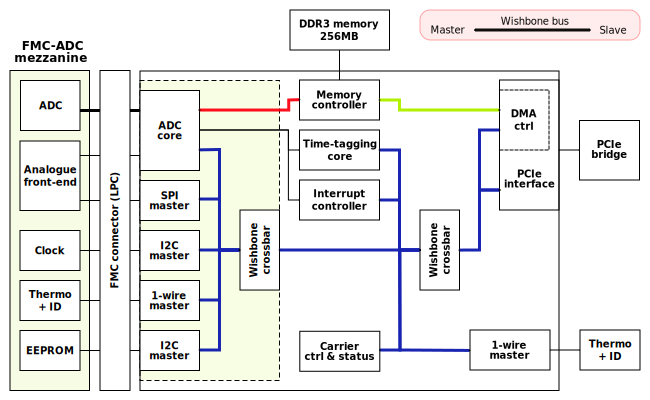
\includegraphics[height=6.5cm]{../paper/figures/spec-fmc-adc_arch.eps}
  \end{center}

\end{frame}

%============ SUB-SECTION ============================================
\subsection{New tools and concepts}

%------------ FRAME --------------------------------------------------
\begin{frame}{Tools}

  \begin{block}{hdlmake}
    \begin{itemize}
    \item
      Project structure descibed in \textit{Manifest} files
    \item
      Solves dependencies
    \item
      Generates \textit{Makefile} for synthesis and simulation
    \end{itemize}
  \end{block}

  \begin{block}{wbgen2}
    \begin{itemize}
    \item
      Wishbone slave generator
    \item
      Structure described in a text file
    \item
      hdl, C header and documentation automatically generated
    \end{itemize}
  \end{block}

\end{frame}

%------------ FRAME --------------------------------------------------
\begin{frame}{New concepts}

  \begin{block}{Self Describing Bus}
    \begin{itemize}
    \item
      
    \item
      
    \item
      
    \end{itemize}
  \end{block}

  \begin{block}{SDB File System}
    \begin{itemize}
    \item
      
    \item
      
    \item
      
    \end{itemize}
  \end{block}

\end{frame}

%------------ FRAME --------------------------------------------------
\begin{frame}[fragile]{SDB record example}

  %\begin{block}{SDB record example}
    \begin{verbatim}
      constant c_ONEWIRE_SDB_DEVICE : t_sdb_device := (
         abi_class     => x"0000",
         abi_ver_major => x"01",
         abi_ver_minor => x"01",
         wbd_endian    => c_sdb_endian_big,
         wbd_width     => x"4",
         sdb_component => (
         addr_first  => x"0000000000000000",
         addr_last   => x"0000000000000007",
         product     => (
            vendor_id => x"000000000000CE42",
            device_id => x"00000602",
            version   => x"00000001",
            date      => x"20121116",
            name      => "WB-Onewire.Control ")));
    \end{verbatim}
  %\end{block}

\end{frame}

%============ SUB-SECTION ============================================
\subsection{Boards}

%------------ FRAME --------------------------------------------------
\begin{frame}{Carrier boards}

  \begin{block}{Fully supported}
    \begin{itemize}
    \item
      SPEC
    \item
      SVEC
    \item
      SPEXI
    \end{itemize}
  \end{block}

  \begin{block}{Other carriers}
    \begin{itemize}
    \item
      VFC
    \item
      PFC
    \item
      AFC
    \item
      RHINO
    \item
      VXS DSP carrier
    \item
      Stand-alone 18-slot FMC carrier
    \end{itemize}
  \end{block}

\end{frame}

%------------ FRAME --------------------------------------------------
\begin{frame}{Mezzanine boards}

  \begin{block}{Fully supported}
    \begin{itemize}
    \item
      ADC-100M
    \item
      TDC
    \item
      DIO-5ch
    \item
      FD
    \end{itemize}
  \end{block}

  \begin{block}{Other mezzanines}
    \begin{itemize}
    \item
      ADC-130M, ADC-200k, ADC-250M, ADC-1G
    \item
      ADC-125M-DAC-600M, ADC-10M-DAC-50M
    \item
      DAC-10M, DAC-130M, DAC-250M, DAC-600M-DDS
    \item
      DIO-16ch, DIO-32ch
    \item
      + others more specific mezzanines
    \end{itemize}
  \end{block}

\end{frame}

%------------ FRAME --------------------------------------------------
\begin{frame}{Easy porting}

  \begin{block}{}
    \begin{itemize}
    \item
      ADC-100M on SPEC = few months
    \item
      2x ADC-100M on SVEC = one week
    \end{itemize}
  \end{block}

\end{frame}


%############ SECTION ################################################
\section{Open Hardware}

%============ SUB-SECTION ============================================
\subsection{Benefits}

%------------ FRAME --------------------------------------------------
%\begin{frame}{}
%  \begin{block}{}
%    \begin{itemize}
%    \item
%    \item
%    \item
%    \end{itemize}
%  \end{block}
%\end{frame}

%============ SUB-SECTION ============================================
\subsection{Collaborations}

%------------ FRAME --------------------------------------------------
%\begin{frame}{}
%  \begin{block}{}
%    \begin{itemize}
%    \item
%    \item
%    \item
%    \end{itemize}
%  \end{block}
%\end{frame}

%============ SUB-SECTION ============================================
\subsection{Drawbacks}

%------------ FRAME --------------------------------------------------
%\begin{frame}{}
%  \begin{block}{}
%    \begin{itemize}
%    \item
%    \item
%    \item
%    \end{itemize}
%  \end{block}
%\end{frame}


%############ SECTION ################################################
\section{Perspectives}

%------------ FRAME --------------------------------------------------
%\begin{frame}{}
%  \begin{block}{}
%    \begin{itemize}
%    \item
%    \item
%    \item
%    \end{itemize}
%  \end{block}
%\end{frame}

%############ SECTION ################################################
\section{Conclusions}

%------------ FRAME --------------------------------------------------
%\begin{frame}{}
%  \begin{block}{}
%    \begin{itemize}
%    \item
%    \item
%    \item
%    \end{itemize}
%  \end{block}
%\end{frame}


%------------ FRAME --------------------------------------------------
%\begin{frame}{}
%  \begin{block}{}
%    \begin{itemize}
%    \item
%    \item
%    \item
%    \end{itemize}
%  \end{block}
%\end{frame}



%\vspace{0.2cm}
%Opening up your designs does make you more vulnerable to this disease.
%\end{frame}
%%One slide to justify our license choice so far
%% One slide on evil patents and the risk for open design.

\end{document}


